\begin{name}
	{Nhóm \LaTeX\ PT THỦ ĐÔ}
	{KIỂM TRA CUỐI HỌC KỲ II LỚP 12 THPT}
\end{name}

\Opensolutionfile{ansbook}[ans/ansb\currfilebase]

%======== PHẦN I. TRẮC NGHIỆM (NHIỀU PHƯƠNG ÁN) ========

\caulc
\Opensolutionfile{ans}[ans/ans\currfilebase-Phan-I]

%Câu 1 (TN)
\begin{ex}%%[2H5N3-2]
	Trong không gian $Oxyz$, mặt cầu $(S)\colon(x-3)^2+(y+1)^2+z^2=36$ có bán kính bằng
	\choice
	{$4$}
	{$16$}
	{\True $6$}
	{$9$}
	\loigiai{Mặt cầu $(S)\colon(x-3)^2+(y+1)^2+z^2=36$ có bán kính bằng $6$.}
\end{ex}

%Câu 2 (TN)
\begin{ex}%%[bỏ]%%
	Các nghiệm của phương trình $z^2+9=0$ trên tập số phức là
	\choice
	{$z=3$ và $z=-3$}
	{$z=i$ và $z=-i$}
	{$z=81i$ và $z=-81i$}
	{\True $z=3i$ và $z=-3i$}
	\loigiai{Ta có $z^2+9=0\Leftrightarrow\hoac{&z=3i\\&z=-3i.}$}
\end{ex}

%Câu 3 (TN)
\begin{ex}%%[2H5H2-1]
	Trong không gian $Oxyz$, đường thẳng $d\colon\heva{&x=1-t\\&y=-3+2t\\&z=2+3t}$ đi qua điểm nào dưới đây?
	\choice
	{\True Điểm $M(1;-3;2)$}
	{Điểm $P(1;2;3)$}
	{Điểm $N(2;-2;-3)$}
	{Điểm $Q(2;2;1)$}
	\loigiai{Đường thẳng $d\colon\heva{&x=1-t \\&y=-3+2t \\&z=2+3t}$ đi qua điểm $M(1;-3;2)$.}
\end{ex}

%Câu 4 (TN)
\begin{ex}%%[2D4N1-1]
	Cho $f(x)$ và $g(x)$ là hai hàm số liên tục trên $\mathbb{R}$. Khẳng định nào dưới đây \textbf{sai}?
	\choice
	{$\displaystyle\int\big[f(x)-g(x)\big]  \mathrm{\,d}x
		=\displaystyle\int f(x)\mathrm{\,d}x-\displaystyle\int g(x)\mathrm{\,d}x$}
	{$\displaystyle\int\big[f(x)+g(x)\big]  \mathrm{\,d}x=\displaystyle\int f(x)\mathrm{\,d} x+\displaystyle\int g(x)\mathrm{\,d} x$}
	{\True $\displaystyle\int\big[f(x)\cdot g(x)\big]  \mathrm{\,d}x=\displaystyle\int f(x)\mathrm{\,d}x \cdot \displaystyle\int g(x) \mathrm{\,d}x$}
	{$\displaystyle\int k \cdot f(x) \mathrm{\,d}x
		=k\displaystyle\int f(x)\mathrm{\,d}x$ $(k\neq 0)$}
	\loigiai{Khẳng định \textbf{sai} là $\displaystyle\int\big[f(x)\cdot g(x)\big]  \mathrm{\,d}x=\displaystyle\int f(x)\mathrm{\,d}x \cdot\displaystyle\int g(x)\mathrm{\,d}x$.}
\end{ex}

%Câu 5 (TN)
\begin{ex}%[BỎ]
	Điểm $M(3;-4)$ là điểm biểu diễn hình học cho số phức nào dưới đây?
	\choice
	{$z=-4+3i$}
	{$z=-3+4i$}
	{\True $z=3-4i$}
	{$z=-3-4i$}
	\loigiai{Điểm $M(3;-4)$ là điểm biểu diễn cho số phức $z=3-4i$.}
\end{ex}

%Câu 6 (TN)
\begin{ex}%%[2D4N1-2]
	Hàm số $F(x)$ là một nguyên hàm của hàm số $f(x)$ trên $\mathbb{R}$. Khẳng định nào dưới đây đúng?
	\choice[2]
	{$\displaystyle\int\big[f(x)+3\big]\mathrm{\,d}x=F(x)+3x^3+C$}
	{\True $\displaystyle\int\big[f(x)+3\big]\mathrm{\,d}x=F(x)+3x+C$}
	{$\displaystyle\int\big[f(x)+3\big]\mathrm{\,d}x=F(x)+x^3+C$}
	{$\displaystyle\int\big[f(x)+3\big]\mathrm{\,d}x=F(x)+C$}
	\loigiai{Ta có $\displaystyle\int\big[f(x)+3\big]\mathrm{\,d}x=\displaystyle\int f(x)\mathrm{\,d}x+\displaystyle\int 3 \mathrm{\,d}x=F(x)+3x+C$.}
\end{ex}

%Câu 7 (TN)
\begin{ex}%[BỎ]
	Cho số phức $z$ thỏa mãn $z(2+i)-13i=1$. Môđun của số phức $z$ bằng
	\choice
	{$\dfrac{\sqrt{34}}{3}$}
	{\True $\sqrt{34}$}
	{$\dfrac{5 \sqrt{34}}{3}$}
	{$34$}
	\loigiai{Ta có $z(2+i)-13i=1\Leftrightarrow z=\dfrac{1+13i}{2+i}=3+5i$.\\
		Vậy $|z|=|3+5i|=\sqrt{3^2+5^2}=\sqrt{34}$.}
\end{ex}

%Câu 8 (TN)
\begin{ex}%[BỎ]
	Phương trình nào dưới đây nhận hai số phức $1+\sqrt{3}i$ và $1-\sqrt{3}i$ là nghiệm?
	\choice
	{$z^2+2z+4=0$}
	{$z^2-2z-4=0$}
	{\True $z^2-2z+4=0$}
	{$z^2+2z-4=0$}
	\loigiai{Ta có $z^2-2z+4=0\Leftrightarrow\hoac{&z=1+\sqrt{3}i\\&z=1-\sqrt{3}i.}$}
\end{ex}

%Câu 9 (TN)
\begin{ex}%%[2D4N3-1]
	Diện tích hình phẳng giới hạn bởi hai đường thẳng $x=0$, $x=\pi$, đồ thị hàm số $y=\cos x$ và trục $Ox$ là
	\choice
	{$S=\displaystyle\int\limits_0^\pi\cos x\mathrm{\,d}x$}
	{\True $S=\displaystyle\int\limits_0^\pi|\cos x| \mathrm{\,d}x$}
	{$S=\displaystyle\int\limits_0^\pi \cos ^2 x \mathrm{\,d}x$}
	{$S=\pi \displaystyle\int\limits_0^\pi|\cos x| \mathrm{\,d}x$}
	\loigiai{Diện tích hình phẳng giới hạn bởi hai đường thẳng $x=0$, $x=\pi$, đồ thị hàm số $y=\cos x$ và trục $Ox$ là $S=\displaystyle\int\limits_0^\pi|\cos x| \mathrm{\,d}x$.}
\end{ex}

%Câu 10 (TN)
\begin{ex}%%[2D4N2-1]
	Nếu $\displaystyle\int\limits_0^1 f(x)\mathrm{\,d}x=2$ thì $\displaystyle\int\limits_1^0 f(x)\mathrm{\,d}x$ bằng
	\choice
	{$1$}
	{\True $-2$}
	{$2$}
	{$-1$}
	\loigiai{Ta có $\displaystyle\int\limits_1^0 f(x) \mathrm{\,d}x=-\displaystyle\int\limits_0^1 f(x) \mathrm{\,d}x=-2$.}
\end{ex}

%Câu 11 (TN)
\begin{ex}%[BỎ]
	Môđun của số phức $z=(3+4i)(1-2i)$ bằng
	\choice
	{$25\sqrt{5}$}
	{$25$}
	{$5$}
	{\True $5\sqrt{5}$}
	\loigiai{
		Ta có $z=(3+4i)(1-2i)=3-6i+4i-8i^2=11-2i$.\\
		Do đó $|z|=\sqrt{11^2+(-2)^2}=5\sqrt{5}$.	
	}
\end{ex}

%Câu 12 (TN)
\begin{ex}%%[2H5N2-2]
	Trong không gian $Oxyz$, cho đường thẳng $d\colon \dfrac{x-1}{2}=\dfrac{y+3}{1}=\dfrac{z-1}{-1}$. Vectơ nào sau đây là một vectơ chỉ phương của $d$?
	\choice
	{$\overrightarrow{u}_1=(2;1;1)$}
	{$\overrightarrow{u}_4=(2;3;-1)$}
	{$\overrightarrow{u}_2=(1;-3;1)$}
	{\True $\overrightarrow{u}_3=(2;1;-1)$}
	\loigiai{
		Vectơ chỉ phương của $d$ là $\overrightarrow{u}_3=(2;1;-1)$.
	}
\end{ex}

%Câu 13 (TN)
\begin{ex}%%[2D4H1-4]
	Cho hàm số $f(x)=4x^3+\mathrm{e}^x$. Khẳng định nào dưới đây đúng?
	\choice
	{\True $\displaystyle\int f(x) \mathrm{\,d}x=x^4+\mathrm{e}^x+C$}
	{$\displaystyle\int f(x) \mathrm{\,d}x=\dfrac{x^4}{4}+\mathrm{e}^x+C$}
	{$\displaystyle\int f(x) \mathrm{\,d}x=x^4+\dfrac{\mathrm{e}^{x+1}}{x+1}+C$}
	{$\displaystyle\int f(x) \mathrm{\,d}x=12x^2+\mathrm{e}^x+C$}
	\loigiai{
		Ta có $\displaystyle\int f(x) \mathrm{\,d}x=\displaystyle\int \left(4x^3+\mathrm{e}^x\right)\mathrm{d}x=x^4+\mathrm{e}^x+C$.
	}
\end{ex}

%Câu 14 (TN)
\begin{ex}%%[2D4H2-1]
	Nếu $\displaystyle\int\limits_{-2}^1 f(x)\mathrm{\,d}x=4$ và $\displaystyle\int\limits_{-2}^1 g(x)\mathrm{\,d}x=-4$ thì $\displaystyle\int\limits_{-2}^1\big[f(x)-g(x)\big]\mathrm{\,d}x$ bằng
	\choice
	{$1$}
	{$-2$}
	{$0$}
	{\True $8$}
	\loigiai{
		Ta có $\displaystyle\int\limits_{-2}^1\big[f(x)-g(x)\big] \mathrm{\,d}x=\displaystyle\int\limits_{-2}^1 f(x) \mathrm{\,d}x-\displaystyle\int\limits_{-2}^1 g(x) \mathrm{\,d}x=4-(-4)=8$.
	}
\end{ex}

%Câu 15 (TN)
\begin{ex}%%[2H5H1-1]
	Trong không gian $Oxyz$, cho mặt phẳng $(P)\colon 3x+y+z-3=0$. Điểm nào dưới đây \textbf{không} thuộc mặt phẳng $(P)$?
	\choice
	{$Q(0;0;3)$}
	{$P(0;3;0)$}
	{\True $M(1;1;1)$}
	{$N(1;0;0)$}
	\loigiai{
		Do $3\cdot 1+1+1-3=2\ne 0$ nên điểm $M(1;1;1)$ không thuộc mặt phẳng $(P)$.
	}
\end{ex}

%Câu 16 (TN)
\begin{ex}%[2H5N3-1]
	Diện tích của mặt cầu bán kính $r$ được tính theo công thức nào dưới đây?
	\choice
	{\True $S=4\pi r^2$}
	{$S=8\pi r^2$}
	{$S=\dfrac{4}{3}\pi r^2$}
	{$S=4\pi r^3$}
	\loigiai{
		Diện tích của mặt cầu có bán kính $r$ là $S=4\pi r^2$.
	}
\end{ex}

%Câu 17 (TN)
\begin{ex}%[BỎ]
	Cho số phức $z=3-2i$. Điểm biểu diễn số phức liên hợp của $z$ có tọa độ là
	\choice
	{$(-3;-2)$}
	{$(-3;2)$}
	{\True $(3;2)$}
	{$(3;-2)$}
	\loigiai{
		Ta có $\overline{z}=3+2i$, suy ra điểm biểu diễn của $\overline{z}$ có tọa độ là $M(3;2)$.	
	}
\end{ex}

%Câu 18 (TN)
\begin{ex}%%[2H5H2-2]
	Trong không gian $Oxyz$, cho điểm $A(1;-1;3)$, $B(4;1;-1)$. Đường thẳng $AB$ có một vectơ chỉ phương là
	\choice
	{$\overrightarrow{u}_4=(1;1;4)$}
	{\True $\overrightarrow{u}_1=(3;2;-4)$}
	{$\overrightarrow{u}_3=(4;1;-1)$}
	{$\overrightarrow{u}_2=(1;-1;3)$}
	\loigiai{
		Đường thẳng $AB$ có một vectơ chỉ phương là $\overrightarrow{AB}=(3;2;-4)$.
	}
\end{ex}

%Câu 19 (TN)
\begin{ex}%%[2D4N3-3]
	Cho hàm số $y=f(x)$ liên tục trên đoạn $[a;b]$. Gọi $D$ là hình phẳng giới hạn bởi đồ thị hàm số $y=f(x)$, trục hoành và hai đường thẳng $x=a$, $x=b$ ($a<b$). Thể tích của khối tròn xoay tạo thành khi quay $D$ quanh trục hoành là
	\choice
	{$V=\pi^2 \displaystyle\int\limits_a^b f(x) \mathrm{\,d}x$}
	{\True $V=\pi \displaystyle\int\limits_a^b f^2(x) \mathrm{\,d}x$}
	{$V=\pi^2\displaystyle\int\limits_a^b f^2(x) \mathrm{\,d}x$}
	{$V=\displaystyle\int\limits_a^b\big|f(x)\big|\mathrm{\,d}x$}
	\loigiai{
		Thể tích của khối tròn xoay tạo thành khi quay $D$ quanh trục hoành là $V=\pi \displaystyle\int\limits_a^b f^2(x)\mathrm{\,d}x$.
	}
\end{ex}

%Câu 20 (TN)
\begin{ex}%[BỎ]
	Cho $z_1=1+2i$, $z_2=-3+2i$. Kết quả phép tính $z_1+z_2$ là
	\choice
	{$-2-i$}
	{$-2-4i$}
	{$2+4i$}
	{\True $-2+4i$}
	\loigiai{
		Ta có $z_1+z_2=1+2i-3+2i=-2+4i$.	
	}
\end{ex}

%Câu 21 (TN)
\begin{ex}%%[2H5H1-3]
	Trong không gian $Oxyz$, cho ba điểm $A(3; 0; 0)$, $B (0; 2; 0)$ và $C(0; 0; 2)$. Mặt phẳng $(ABC)$ có phương trình là
	\choice
	{\True $\dfrac{x}{3}+\dfrac{y}{2}+\dfrac{z}{2}=1$}
	{$\dfrac{x}{3}+\dfrac{y}{2}+\dfrac{z}{2}=-1$}
	{$\dfrac{x}{3}+\dfrac{y}{2}+\dfrac{z}{2}=0$}
	{$\dfrac{x}{3}+\dfrac{y}{1}+\dfrac{z}{2}=1$}	
	\loigiai{Mặt phẳng $(ABC)$ đi qua ba điểm $A(3; 0; 0)$, $B(0; 2; 0)$, $C(0; 0; 2)$ nên có phương trình mặt phẳng chắn là $\dfrac{x}{3}+\dfrac{y}{2}+\dfrac{z}{2}=1$. 
	}
\end{ex}

%Câu 22 (TN)
\begin{ex}%%[2H5N1-2]
	Trong không gian $Oxyz$, mặt phẳng $(P)\colon 2x+3y-5z-1=0$ có một vectơ pháp tuyến có tọa độ là	
	\choice
	{$(2;3;-4)$}
	{$(-2;3;5)$}
	{\True $(2;3;-5)$}
	{$(2;3;5)$}	
	\loigiai{ 
		Mặt phẳng $(P)\colon 2x+3y-5z-1=0$ có một vectơ pháp tuyến là $\overrightarrow{n}_{(P)}=(2;3;-5)$.
	}
\end{ex}

%Câu 23 (TN)
\begin{ex}%%[2D4H2-1]
	Cho hàm số $f(x)$ có $f(1)=1$, $f(3)=5$, hàm số $f'(x)$ liên tục trên đọạn $[1;3]$. Khi đó $\displaystyle\int\limits_1^3 f'(x)\mathrm{\,d}x$ bằng
	\choice
	{$-2$}
	{$-4$}
	{\True $4$}
	{$2$}	
	\loigiai{ 
		Ta có $\displaystyle\int\limits_1^3 f'(x)\mathrm{\,d}x=f(x)\Big|_1^3=f(3)-f(1)=5-1=4$.
	}
\end{ex}

%Câu 24 (TN)
\begin{ex}%%[2H2H2-2]
	Trong không gian $Oxyz$, hình chiếu vuông góc của điểm $M(-1;-2;3)$ trên mặt phẳng $(Oxz)$ có tọa độ là
	\choice
	{\True $(-1;0;3)$}
	{$(3;-1;0)$}
	{$(-1;3;0)$}
	{$(-1;0;2)$}	
	\loigiai{
		Hình chiếu vuông góc của điểm $M(-1;-2;3)$ trên mặt phẳng $(Oxz)$ có tọa độ là $M(-1;0;3)$.
	}
\end{ex}

%Câu 25 (TN)
\begin{ex}%[BỎ]
	Cho hai số phức $z_1=-1+2 i$ và $z_2=5+7i$. Số phức $z_1-z_2$ có phần ảo bằng
	\choice
	{\True $-5$}
	{$4$}
	{$-5i$}
	{$-4$}	
	\loigiai{
		Ta có $z_1-z_2=(-1+2i)-(5+7i)=-6-5i$ nên có phần ảo là $-5$.
	}
\end{ex}

%Câu 26 (TN)
\begin{ex}%[BỎ]
	Cho số phức $z=-3+4 i$. Môđun của số phức $z$ bằng
	\choice
	{\True $5 $}
	{$\sqrt{7}$}
	{$25$}
	{$1$}	
	\loigiai{
		$|z|=|-3+4i|=\sqrt{(-3)^3+4^2}=5$.
	}
\end{ex}

%Câu 27 (TN)
\begin{ex}%%[2D4H3-1]
	Cho hàm số $y=f(x)$ liên tục trên $[0;2]$ và bảng xét dấu như sau:
	\begin{center}
		
\begin{tikzpicture}[font=\normalsize,t style/.style={style=solid}]
			%dòng khai báo
			\tkzTabInit[nocadre=true, lgt=1.2, espcl=4, deltacl=0.5]
			{$x$/ 0.7,$f(x)$/0.7}
			{$0$,$1$,$2$}
			%dòng xét dấu thứ 1
			\tkzTabLine{,+, 0, -,} 
		\end{tikzpicture}
	\end{center}	
	Diện tích hình phẳng giới hạn bởi đồ thị $y=f(x)$, trục hoành và hai đường thẳng $x=0$, $x=2$ là
	\choice
	{$S=\left|\displaystyle\int\limits_0^2 f(x)\mathrm{\,d}x\right|$}
	{$S=-\displaystyle\int\limits_0^1 f(x)\mathrm{\,d}x+\displaystyle\int\limits_1^2 f(x)\mathrm{\,d}x$}
	{\True $S=\displaystyle\int\limits_0^1 f(x)\mathrm{\,d}x-\displaystyle\int\limits_1^2 f(x)\mathrm{\,d}x$}
	{$S=\displaystyle\int\limits_0^2 f(x)\mathrm{\,d}x$}	
	\loigiai{
		Diện tích hình phẳng giới hạn bởi đồ thị $y=f(x)$, trục hoành và hai đường thẳng $x=0, x=2$ được tính theo công thức $S=\displaystyle\int\limits_0^2\big|f(x)\big|\mathrm{\,d}x
		=\displaystyle\int\limits_0^1 \big|f(x)\big|\mathrm{\,d}x+\displaystyle\int\limits_1^2\big|f(x)\big|\mathrm{\,d}x
		=\displaystyle\int\limits_0^1 f(x)\mathrm{\,d}x-\displaystyle\int\limits_1^2 f(x)\mathrm{\,d}x$.
	}
\end{ex}

%Câu 28 (TN)
\begin{ex}%%[2H2N2-3]
	Trong không gian $Oxyz$, cho hai điểm $A(1;1;2)$ và $B(4;2;3)$. Vectơ $\overrightarrow{AB}$ có tọa độ là
	\choice
	{$(-1;3;1)$}
	{\True $(3;1;1)$}
	{$(1;1;1)$}
	{$(3;2;1)$}	
	\loigiai{
		Vectơ $\overrightarrow{AB}=(3;1;1)$.
	}
\end{ex}

%Câu 29 (TN)
\begin{ex}%[BỎ]
	Cho hàm số $f(x)=x\cos x$. Khẳng định nào dưới đây đúng?
	\choice
	{$\displaystyle\int f(x)\mathrm{\,d}x=x\sin x-\cos x+C$}
	{$\displaystyle\int f(x)\mathrm{\,d}x=\dfrac{x^2}{2}\sin x+C$}
	{$\displaystyle\int f(x)\mathrm{\,d}x=-x\sin x-\cos x+C$}
	{\True $\displaystyle\int f(x)\mathrm{\,d}x=x\sin x+\cos x+C$}	
	\loigiai{
		Xét $\displaystyle\int f(x)\mathrm{\,d}x=\displaystyle\int x\cos x\mathrm{\,d}x$. Đặt $\heva{&u=x\\&\mathrm{d}v=\cos x\mathrm{\,d}x}\Rightarrow \heva{&\mathrm{d}u=\mathrm{\,d}x\\&v=\sin x.}$\\
		Suy ra $\displaystyle\int f(x)\mathrm{\,d}x=x\sin x-\displaystyle\int\sin x \mathrm{\,d}x=x\sin x+\cos x+C$.
	}
\end{ex}

%Câu 30 (TN)
\begin{ex}%%[2H2N2-3]
	Trong không gian $Oxyz$, cho hai vectơ $\overrightarrow{u}=(-2;3;2)$ và $\overrightarrow{v}=(3;2;-1)$. Tọa độ của vectơ $\overrightarrow{u}+\overrightarrow{v}$ là
	\choice
	{$(-2;3;2)$}
	{\True $(1;5;1)$}
	{$(1;-5;-1)$}
	{$(3;2;-1)$}	
	\loigiai{ 
		Ta có $\overrightarrow{u}+\overrightarrow{v}=(1;5;1)$.
	}
\end{ex}

%Câu 31 (TN)
\begin{ex}%%[2D4H3-1]
	Diện tích hình phẳng giới hạn bởi các đồ thị hàm số $y=x^2+1$ và $y=3-x^2$ bằng
	\choice
	{$\dfrac{4}{3}$}
	{$\dfrac{2}{3}$}
	{\True $\dfrac{8}{3}$}
	{$0$}	
	\loigiai{Phương trình hoành độ giao điểm của hai đồ thị là $x^2+1=3-x^2\Leftrightarrow x^2-1=0\Leftrightarrow\hoac{&x=1\\&x=-1.}$\\
		Diện tích hình phẳng cần tìm là
		\[\displaystyle\int\limits_{-1}^1\left|x^2+1-3+x^2\right|\mathrm{d}x=\displaystyle\int\limits_{-1}^1\left|2x^2-2\right|\mathrm{d}x=\displaystyle\int\limits_{-1}^1\left(2-2x^2\right)\mathrm{d}x=\dfrac{8}{3}.\]}
\end{ex}

%Câu 32 (TN)
\begin{ex}%%[2H5H2-3]
	Trong không gian $Oxyz$, cho ba điểm $A(2;-3;1)$, $B(1;-3;4)$ và $C(2;-1;2)$. Đường thẳng đi qua $A$ và song song với $BC$ có phương trình là
	\choice
	{$\dfrac{x-2}{1}=\dfrac{y+2}{2}=\dfrac{z-3}{-2}$}
	{$\dfrac{x+2}{1}=\dfrac{y-2}{-4}=\dfrac{z+3}{2}$}
	{\True $\dfrac{x-2}{1}=\dfrac{y+3}{2}=\dfrac{z-1}{-2}$}
	{$\dfrac{x-2}{1}=\dfrac{y+3}{-2}=\dfrac{z-1}{6}$}	
	\loigiai{Đường thẳng đi qua $A(2;-3;1)$ và nhận $\overrightarrow{BC}=(1;2;-2)$ làm vectơ chỉ phương nên có phương trình là $\dfrac{x-2}{1}=\dfrac{y+3}{2}=\dfrac{z-1}{-2}$.}
\end{ex}

%Câu 33 (TN)
\begin{ex}%[BỎ]
	Cho tích phân $I=\displaystyle\int\limits_0^2(x+1)\mathrm{e}^x\mathrm{\,d}x$. Đặt $u=x+1$, $\mathrm{\,d}v=\mathrm{e}^x\mathrm{\,d}x$. Khẳng định nào dưới đây đúng?
	\choice
	{$I=(x+1)\mathrm{e}^x\Big|_0^2-2\displaystyle\int\limits_0^2\mathrm{e}^x\mathrm{\,d}x$}
	{$I=(x+1)\Big|_0^2-\displaystyle\int\limits_0^2\mathrm{e}^x\mathrm{\,d}x$}
	{$I=(x+1)\mathrm{e}^x\Big|_0^2+\displaystyle\int\limits_0^2\mathrm{e}^x\mathrm{\,d}x$}
	{\True $I=(x+1)\mathrm{e}^x\Big|_0^2-\displaystyle\int\limits_0^2\mathrm{e}^x\mathrm{\,d}x$}	
	\loigiai{Đặt $\heva{&u=x+1\\&\mathrm{\,d}v=\mathrm{e}^x\mathrm{\,d}x}\Rightarrow\heva{&\mathrm{\,d}u=\mathrm{\,d}x\\&v=\mathrm{e}^x.}$\\
		Từ đó ta có $I=uv\Big|_0^2-\displaystyle\int\limits_0^2v\mathrm{\,d}u=(x+1)\mathrm{e}^x\Big|_0^2-\displaystyle\int\limits_0^2\mathrm{e}^x\mathrm{\,d}x$.}
\end{ex}

%Câu 34 (TN)
\begin{ex}%[BỎ]
	Gọi $z_0$ là nghiệm phức có phần ảo âm của phương trình $z^2-6z+13=0$. Trên mặt phẳng tọa độ, điểm biểu diễn $1-z_0$ là
	\choice
	{$P(-2;-2)$}
	{$Q(4;-2)$}
	{\True $M(-2;2)$}
	{$N(4;2)$}	
	\loigiai{Ta có $z^2-6z+13=0\Leftrightarrow\hoac{&z=3+2i\\&z=3-2i.}$\\
		Do nghiệm $z_0$ có phần ảo âm nên $z_0=3-2i$.\\
		Vậy điểm biểu diễn của $w=1-z_0=1-(3-2i)=-2+2i$ là $M(-2;2)$.}
\end{ex}

%Câu 35 (TN)
\begin{ex}%[BỎ]
	Gọi $M$, $N$ lần lượt là các điểm biểu diễn của số phức $z=1+i$; $z'=2+4i$. Số phức $w$ có điểm biểu diễn là $Q$ sao cho $\overrightarrow{MN}+2\overrightarrow{MQ}=\overrightarrow{0}$ là
	\choice
	{$w=-\dfrac{1}{2}+\dfrac{1}{2}i$}
	{$w=\dfrac{1}{2}+\dfrac{1}{2}i$}
	{\True $w=\dfrac{1}{2}-\dfrac{1}{2}i$}
	{$w=-\dfrac{1}{2}-\dfrac{1}{2}i$}
	\loigiai{Do $M$, $N$ lần lượt là các điểm biểu diễn của số phức $z=1+i$; $z'=2+4i$ nên $M(1;1)$ và $N(2;4)$.\\
		Ta có $\overrightarrow{MN}+2\overrightarrow{MQ}=\overrightarrow{0}\Leftrightarrow\heva{&x_N-x_M+2(x_Q-x_M)=0\\&y_N-y_M+2(y_Q-y_M)=0}\Leftrightarrow\heva{&x_Q=\dfrac{3x_M-x_N}{2}=\dfrac{1}{2}\\&y_Q=\dfrac{3y_M-y_N}{2}=-\dfrac{1}{2}.}$\\
		Vậy $Q\left(\dfrac{1}{2};-\dfrac{1}{2}\right)$ là điểm biểu diễn của $w=\dfrac{1}{2}-\dfrac{1}{2}i$.}
\end{ex}

%Câu 36 (TN)
\begin{ex}%%[2H5H3-2]
	Trong không gian $Oxyz$, cho mặt cầu $(S)\colon x^2+y^2+z^2-4x+6y-2z+5=0$. Tâm của $(S)$ có tọa độ là
	\choice
	{$(2;3;1)$}
	{$(3;-1;2)$}
	{$(3;2;-1)$}
	{\True $(2;-3;1)$}
	\loigiai{Tâm của $(S)$ là $I(2;-3;1)$.}
\end{ex}

%Câu 37 (TN)
\begin{ex}%%[2H5H1-5]
	Trong không gian $Oxyz$, khoảng cách từ điểm $M(2;-1;3)$ đến mặt phẳng \break $(P)\colon 2x+y-2z+5=0$ bằng
	\choice
	{\True $\dfrac{2}{3}$}
	{$\dfrac{4}{3}$}
	{$2$}
	{$3$}
	\loigiai{Khoảng cách từ $M$ đến $(P)$ là $\mathrm{d}\big(M,(P)\big)=\dfrac{|2\cdot2+(-1)-2\cdot3+5|}{\sqrt{2^2+1^2+(-2)^2}}=\dfrac{2}{3}$.}
\end{ex}

%Câu 38 (TN)
\begin{ex}%[2H5H3-2]
	Cho mặt cầu có diện tích bằng $8\pi$. Khi đó, bán kính mặt cầu bằng
	\choice
	{$2$}
	{$2\sqrt{2}$}
	{\True $\sqrt{2}$}
	{$\dfrac{\sqrt{2}}{2}$}
	\loigiai{Ta có diện tích mặt cầu là $8\pi$ nên $4\pi R^2=8\pi\Leftrightarrow R^2=2\Leftrightarrow R=\sqrt{2}$.}
\end{ex}

%Câu 39 (TN)
\begin{ex}%[BỎ]
	Biết phương trình $z^2+az+b=0$, ($a$, $b\in\mathbb{R})$ có một nghiệm phức là $z_1=1-2i$. Khẳng định nào sau đây là đúng?
	\choice
	{\True $ab=-10$}
	{$a+b=-3$}
	{$a^2-b^2=21$}
	{$2a+b=-1$}
	\loigiai{Do $z_1=1-2i$ là nghiệm của phương trình nên $z_2=1+2i$ cũng là nghiệm của phương trình.\\
		Ta có $\heva{&z_1+z_2=-a\\&z_1z_2=b}\Leftrightarrow\heva{&2=-a\\&5=b}\Leftrightarrow\heva{&a=-2\\&b=5.}$\\
		Suy ra khẳng định đúng là $ab=-10$.}
\end{ex}

%Câu 40 (TN)
\begin{ex}%%[2H5H3-3]
	Trong không gian $Oxyz$, mặt cầu có tâm $I(3;0;0)$ và đi qua điểm $M(0;4;0)$ có phương trình là
	\choice
	{$(x-3)^2+y^2+z^2=5$}
	{$(x+3)^2+y^2+z^2=25$}
	{$(x+3)^2+y^2+z^2=5$}
	{\True $(x-3)^2+y^2+z^2=25$}
	\loigiai{Do mặt cầu có tâm $I$ và đi qua điểm $M$ nên có bán kính là $R=IM=\sqrt{3^2+4^2}=5$.\\
		Phương trình của mặt cầu là $(x-3)^2+y^2+z^2=25$.}
\end{ex}

%Câu 41 (TN)
\begin{ex}%%[2H5H2-3]
	Trong không gian $Oxyz$, cho điểm $M(-1;2;3)$ và mặt phẳng $(P)\colon x-3y+2z+5=0$. Phương trình của đường thẳng đi qua $M$ và vuông góc với $(P)$ là
	\def\dotEX{}
	\choice
	{\True $\heva{&x=t\\&y=-1-3t\\&z=5+2t.}$}
	{$\heva{&x=-1+t\\&y=-2-3t\\&z=3+2t.}$}
	{$\heva{&x=-1+t\\&y=2-3t\\&z=3-2t.}$}
	{$\heva{&x=1+t\\&y=2-3t\\&z=3+2t.}$}
	\loigiai{ 
		Vì $d\perp(P)$ nên vectơ pháp tuyến của mmawjt phẳng $(P)$ chính là vectơ chỉ phương của $d$  hay\break $\overrightarrow{u}_d$=$\overrightarrow{n}_{(P)}=(1;-3;2)$.\\
		Khi đó, đường thẳng $d$ có phương trình tham số là $\heva{&x=t\\&y=-1-3t\\&z=5+2t.}$
	}
\end{ex}

%Câu 42 (TN)
\begin{ex}%[BỎ]
	Thể tích khối cầu ngoại tiếp hình hộp chữ nhật có ba kích thước bằng $1$; $2$; $3$ là	
	\choice
	{$36\pi$}
	{$\dfrac{9\pi}{8}$}
	{$\dfrac{9\pi}{2}$}
	{\True $\dfrac{7\sqrt{14}\pi}{3}$}	
	\loigiai{ 
		\begin{center}
			\begin{tikzpicture}[font=\footnotesize, scale=.7]
				\def\a{3}
				\def\b{2}
				\def\h{3.5}
				\path(0:0) coordinate (A)
				++(0:\a) coordinate (D)
				++(-130:\b) coordinate (C)
				($(A)+(C)-(D)$) coordinate (B)
				($(A)+(90:\h)$) coordinate (A')
				($(B)+(90:\h)$) coordinate (B')
				($(C)+(90:\h)$) coordinate (C')
				($(D)+(90:\h)$) coordinate (D')
				($(A')!.5!(C)$) coordinate (I);
				\draw[dashed] 	(B)--(A)--(D)	(A)--(A')--(C);
				\draw	(C)--(C') 	(D)--(D') 	(B)--(B')	(C)--(C')
				(B)--(C)--(D) 
				(A')--(B')--(C')--(D')--cycle;
				\foreach \x/\g in {A/180,B/180,C/0,D/0,A'/180,B'/180,C'/0,D'/0,I/20}
				\fill 	(\x) circle (1pt)
				($(\g:4mm)+(\x)$) node {$\x$};	
			\end{tikzpicture}
		\end{center}
		Mặt cầu ngoại tiếp hình hộp chữ nhật có
		\begin{itemize}
			\item Tâm là trung điểm đường chéo $A'C$.
			\item Bán kính $R=\dfrac{1}{2}AC'=\dfrac{1}{2}\sqrt{1^2+2^2+3^2}=\dfrac{\sqrt{14}}{2}$.
		\end{itemize} 
		Khi đó, thể tích khối cầu ngoại tiếp hình chữ nhật là $V=\dfrac{4}{3}\pi\left(\dfrac{\sqrt{14}}{2}\right)^3=\dfrac{7\sqrt{14}\pi}{3}$.
	}
\end{ex}

%Câu 43 (TN)
\begin{ex}%[BỎ]
	Gọi $S$ là tổng các số thực $m$ để phương trình $z^2-4 z+4-m=0$ có nghiệm phức thỏa mãn $|z|=3$. Khi đó $S$ bằng
	\choice
	{$20$}
	{\True $21$}
	{$-4$}
	{$26$}	
	\loigiai{Ta có
		$z^2-4z+4-m=0\Leftrightarrow(z-2)^2=m$. $\qquad (1)$
		\begin{itemize}
			\item Trường hợp $1$: $m\geq 0$, ta có $(1)\Leftrightarrow\hoac{&z-2=\sqrt{m}\\&z-2=-\sqrt{m}}
			\Leftrightarrow\hoac{&{z=2+\sqrt{m}}\\&z=2-\sqrt{m}.}$
			\begin{itemize}
				\item Với $z=2+\sqrt{m}\Rightarrow |z|=\left|2+\sqrt{m}\right|=2+\sqrt{m}\Leftrightarrow 2+\sqrt{m}=3\Leftrightarrow \sqrt{m}=1\Leftrightarrow m=1$.
				\item Với $z=2-\sqrt{m}$, suy ra
				\allowdisplaybreaks \begin{eqnarray*}
					&&|z|=\left|2-\sqrt{m}\right|
					\\
					&\Leftrightarrow&\hoac{&2-\sqrt{m}=3\\&2-\sqrt{m}=-3}
					\\
					&\Leftrightarrow& \hoac{&\sqrt{m}=5\\&\sqrt{m}=-1\ \text{(vô nghiệm)}}
					\\
					&\Leftrightarrow& m=25.			 
				\end{eqnarray*}
			\end{itemize}
			\item Trường hợp $2$: $m<0$\\
			$(1)\Leftrightarrow\hoac{&z-2=i\sqrt{-m}\\&z-2=-i\sqrt{-m}}\Leftrightarrow\hoac{&z=2+i \sqrt{-m}\\&z=2-i\sqrt{-m}}\Rightarrow |z|=\sqrt{2^2-m}=\sqrt{4-m}$.\\
			Ta có $|z|=3\Leftrightarrow \sqrt{4-m}=3\Leftrightarrow 4-m=9\Leftrightarrow m=-5$.
		\end{itemize}
		Vậy $S=1+25-5=21$.
	}
\end{ex}

%Câu 44 (TN)
\begin{ex}%%[2D4H2-6]
	Một vật chuyển động chậm dần đều với vận tốc $v(t)=180-10t$ (m/s) trong đó $t$ là thời gian tính bằng giây kể từ lúc vật bắt đầu chuyển động chậm dần đều. Trong $5$ giây trước khi dừng hẳn, vật di chuyển được quãng đường bằng
	\choice
	{\True $775 \mathrm{~m}$}
	{$845 \mathrm{~m}$}
	{$100 \mathrm{~m}$}
	{$125 \mathrm{~m}$}	
	\loigiai{
		\begin{itemize}
			\item Ta có vận tốc $v(t)=180-10t$
			\item Suy ra quãng đường $s=\displaystyle\int\limits_0^5 v(t)dt=\left(180-5 t^2\right)\Big|_0^5=180\cdot 5-5^3=775$\,m.
		\end{itemize}
	}
\end{ex}

%Câu 45 (TN)
\begin{ex}%[BỎ]
	Gọi $M$ là điểm biểu diễn của số phức $z$ thỏa mãn $|z-i|=|(1+i)z|$. Tập hợp tất cả các điểm $M$ như vậy là đường tròn có bán kính
	\choice
	{\True $R=\sqrt{2}$}
	{$R=1$}
	{$R=4$}
	{$R=2$}
	\loigiai{Đặt $z=x+yi$, ($x$; $y\in\mathbb{R}$).
		Khi đó, ta có
		\allowdisplaybreaks \begin{eqnarray*}
			& &|z-i|=|(1+i)z|\\
			&\Leftrightarrow&|x+yi-i|=|(1+i)(x+yi)|\\
			&\Leftrightarrow&|x+i(y-1)|=|(x-y)+(x+y)i|\\
			&\Leftrightarrow&\sqrt{x^2+(y-1)^2}=\sqrt{(x-y)^2+(x+y)^2}\\
			&\Leftrightarrow&x^2+y^2-2y+1=2x^2+2y^2\\
			&\Leftrightarrow&x^2+y^2+2y-1=0\\
			&\Leftrightarrow&x^2+(y+1)^2=2.
		\end{eqnarray*}
		Vậy tập hợp các điểm $M$ là đường tròn tâm $I(0;-1)$, bán kính $R=\sqrt{2}$.}
\end{ex}

%Câu 46 (TN)
\begin{ex}%%[2D4C2-2]
	Cho hàm số $f(x)$ liên tục trên $\mathbb{R}$, $f(x) \neq 0$ với mọi $x$ và thỏa mãn $f(1)=-\dfrac{1}{2}$, \break $f'(x)=(2x+1) f^2(x)$. Khi đó $f\left(-\dfrac{1}{2}\right)$ bằng
	\choice
	{$-2$}
	{\True $4$}
	{$2$}
	{$-4$}
	\loigiai{Ta xét  $f'(x)=(2 x+1) f^2(x)\Leftrightarrow -\dfrac{f'(x)}{f^2(x)}=-(2x+1)$.\\
		Lấy nguyên hàm hai vế, ta được
		\allowdisplaybreaks \begin{eqnarray*}
			& &\displaystyle\int -\dfrac{f'(x)}{f^2(x)}\mathrm{\,d}x=\displaystyle\int-(2x+1)\mathrm{\,d}x\\
			&\Leftrightarrow&\dfrac{1}{f(x)}=-x^2-x+C\\
			&\Leftrightarrow&f(x)=\dfrac{1}{-x^2-x+C}.\\
		\end{eqnarray*}
		Mà $f(-1)=-\dfrac{1}{2}$ nên $-\dfrac{1}{2}=\dfrac{1}{-1^2-1+C}
		\Leftrightarrow C=0$.\\
		Do đó $f(x)=\dfrac{1}{-x^2-x}$.\\
		Vậy $f\left(-\dfrac{1}{2}\right)=\dfrac{1}{-\left( -\dfrac{1}{2}\right)^2-\left( -\dfrac{1}{2}\right)}=4 $.}
\end{ex}

%Câu 47 (TN)
\begin{ex}%%[2D4C3-1]
	Xét $f(x)=ax^4+bx^2+c$ $(a$, $b$, $c\in\mathbb{R}$, $a>0)$ sao cho đồ thị hàm số
	$y=f(x)$ có ba điểm cực trị là $A$, $B$ và $C(1;-2)$. Gọi $y=g(x)$ là hàm số bậc
	hai có đồ thị đi qua ba điểm $A$, $B$ và $C$. Khi hình phẳng giới hạn bởi đồ thị
	của hai hàm số $y=f(x)$, $y=g(x)$ và hai đường thẳng $x=0$, $x=1$ có diện tích bằng
	$\dfrac{4}{5}$, tích phân $\displaystyle\int\limits_0^1 f(x)\mathrm{\,d}x$ bằng
	\choice
	{\True $\dfrac{6}{5}$}
	{$-\dfrac{6}{5}$}
	{$1$}
	{$-1$}
	\loigiai{
		Ta có $f'(x)=4ax^3+2bx$.\\
		Vì $y=f(x)=ax^4+bx^2+c$ có điểm cực trị $C(1;-2)$ nên
		\allowdisplaybreaks \begin{eqnarray*}
			\heva{&f(1)=-2\\&f'(1)=0}&\Leftrightarrow&	\heva{&a+b+c=-2\\&4a+2b=0}\\
			&\Leftrightarrow&\heva{&a=c+2\\&b=-2(c+2).}\\
			&\Rightarrow&y=f(x)=(c+2)x^4-2(c+2)x^2+c, \,(c\ne 2).
		\end{eqnarray*}
		Suy ra, đồ thị hàm số có $3$ điểm cực trị là $A(-1;-2)$, $B(0;c)$, $C(1;-2)$.\\
		Vì $y=g(x)=mx^2+nx+p$ là hàm số bậc hai có đồ thị đi qua ba điểm $A(-1;-2)$, $B(0;c)$ và $C(1;-2)$ nên
		\[\heva{&m=-(c+2)\\&n=0\\&p=c.}\]
		Do đó $y=g(x)=-(c+2)x^2+c$.\\
		Vì hình phẳng giới hạn bởi đồ thị của hai hàm số $y=f(x)$, $y=g(x)$ và hai đường
		thẳng \break $x=0$, $x=1$ có diện tích bằng $\dfrac{4}{5}$ nên
		\[\displaystyle\int\limits_0^1\big| g(x)-f(x)\big|\mathrm{\,d}x=\dfrac{4}{5}.\qquad(*)\]
		\begin{center}
			\begin{tikzpicture}[line cap=butt,font=\footnotesize, line join=miter,>=stealth]
				\tikzset{declare function={xmin=-2;xmax=2.5;ymin=-3;ymax=5;
						f(\x)=6*(\x)^4-12*(\x)^2+4;
						g(\x)=-6*(\x)^2+4;
					},
					smooth,samples=450
				}
				\draw[->] (xmin,0)--(xmax,0) node[shift={(-100:7pt)}]{$x$};
				\draw[->] (0,ymin)--(0,ymax) node[shift={(190:7pt)}]{$y$};
				\fill (0,0) circle(1pt) node[shift={(225:7pt)}]{$O$};
				\draw[dashed] (1,0)node[above]{$1$}--(1,-2)--(0,-2)node[below left]{$-2$}--(-1,-2)--(-1,0)node[above]{$-1$} (0,4)node[above left]{$c$}
				;
				\fill (-1,-2) circle(1pt) (-1,0) circle(1pt) (1,0) circle(1pt);
				\fill (1,-2) circle(1pt);
				\fill (0,4) circle(1pt);
				\node at (1.5,4.5)[right]{$y=f(x)$};
				\node at (1.2,-2.6)[right]{$y=g(x)$};
				\clip (xmin,ymin) rectangle (xmax,ymax);
				\draw  plot[domain=xmin:xmax] (\x, {f(\x)});
				\draw[red]  plot[domain=xmin:xmax] (\x, {g(\x)});
				\path[name path=fx] plot[domain=-0.01:1.01] (\x, {f(\x)});
				\path[name path=gx] plot[domain=-0.01:1.01] (\x, {g(\x)});
				\tikzfillbetween[of=fx and gx] {pattern=north west lines};
			\end{tikzpicture}			
		\end{center}
		Dựa vào đồ thị hàm số, ta thấy $g(x)\geq f(x)$, $\forall x\in [0;1]$.  Khi đó 
		\allowdisplaybreaks \begin{eqnarray*}
			(*)&\Leftrightarrow&\displaystyle\int\limits_0^1\big[g(x)-f(x)\big]\mathrm{\,d}x=\dfrac{4}{5}\\
			&\Leftrightarrow&\displaystyle\int\limits_0^1{\left[(c+2)x^2-(c+2)x^4\right]\mathrm{d}x}=\dfrac{4}{5}
			\\
			&\Leftrightarrow&c=4\\
			&\Rightarrow&a=6;b=-12.\\
		\end{eqnarray*}
		Vậy $\displaystyle\int\limits_0^1 f(x)\mathrm{\,d}x
		=\displaystyle\int\limits_0^1\left(6x^4-12x^2+4\right)\mathrm{d}x
		=\dfrac{6}{5}$.
	}
\end{ex}

%Câu 48 (TN)
\begin{ex}%%[2H5V1-3]
	Trong không gian $Oxyz$, cho điểm $A(5;4;2)$ và mặt cầu
	$(S)\colon (x-1)^2+(y-2)^2+z^2=4$. Biết $B$, $C$, $D$ là ba điểm phân biệt trên $(S)$ sao
	cho các tiếp diện của $(S)$ tại mỗi điểm đó đều đi qua $A$. Hỏi mặt phẳng $(BCD)$ đi qua điểm nào dưới đây?
	\choice
	{$N(-1;1;5)$}
	{$Q(1;2;-1)$}
	{\True $M(2;1;1)$}
	{$P(1;1;2)$}
	\loigiai{Mặt cầu $(S)$ có tâm $I(1;2;0)$ và bán kính $R=2$.\\
		Vì $B(x;y;z)$ là tiếp điểm nên $IA^2=IB^2+AB^2\Leftrightarrow AB^2=24-4=20$.\\
		Khi đó $\heva{&(x-1)^2+(y-2)^2+z^2=4\\&(x-5)^2+(y-4)^2+(z-2)^2=20}\Rightarrow
		-8x-4y-4z+40=16$.\\
		Do đó mặt phẳng $(P)\colon 2x+y+z-6=0\Rightarrow M(2;1;1)\in (P)$.
	}
\end{ex}

%Câu 49 (TN)
\begin{ex}%%[2H5C3-3]
	Trong không gian $Oxyz$, cho hai điểm $A(1;0;2)$, $B(1;-1;3)$ và đường thẳng\break $\Delta\colon \dfrac{x+3}{-2}=\dfrac{y-2}{1}=\dfrac{z-1}{-1}$. Mặt phẳng $(P)$ đi qua $B$, vuông góc với $\Delta$ và chứa điểm $M$ thay đổi sao cho tam giác $AMB$ vuông tại $M$. Khi độ dài $M B$ lớn nhất thì độ dài đoạn $OM$ bằng
	\choice
	{\True $\dfrac{5\sqrt{3}}{3}$}
	{$\dfrac{5\sqrt{3}}{2}$}
	{$\sqrt{7}$}
	{$5\sqrt{3}$}	
	\loigiai{
		\begin{center}
			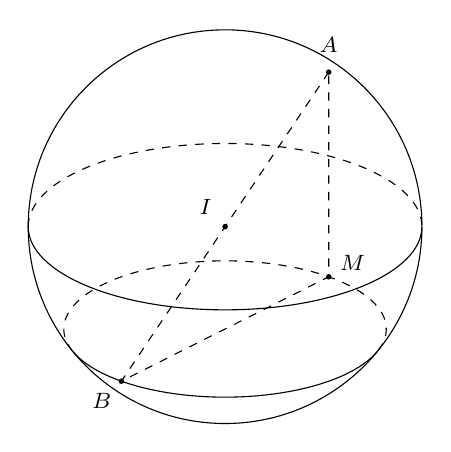
\begin{tikzpicture}[font=\footnotesize,scale=1]
				\newcommand\pgfmathsinandcos[3]{
					\pgfmathsetmacro#1{sin(#3)}
					\pgfmathsetmacro#2{cos(#3)}
				}
				\newcommand\LongitudePlane[2][current plane]{
					\pgfmathsinandcos\sinEl\cosEl{\Elevation} 
					\pgfmathsinandcos\sint\cost{#2} 
					\tikzset{#1/.estyle={cm={\cost,\sint*\sinEl,0,\cosEl,(0,0)}}}
				}
				\newcommand\LatitudePlane[2][current plane]{
					\pgfmathsinandcos\sinEl\cosEl{\Elevation} 
					\pgfmathsinandcos\sint\cost{#2} 
					\pgfmathsetmacro\ydelta{\cosEl*\sint}
					\tikzset{#1/.estyle={cm={\cost,0,0,\cost*\sinEl,(0,\ydelta)}}} 
				}
				\newcommand\DrawLongitudeCircle[1]{
					\LongitudePlane{#1}
					\tikzset{current plane/.prefix style={scale=\R}}
					\pgfmathsetmacro\angVis{atan(sin(#1)*cos(\Elevation)/sin(\Elevation))} 
					\draw[current plane,thin,black]  (\angVis:1)     arc (\angVis:\angVis+180:1);
					\draw[current plane,thin,dashed] (\angVis-180:1) arc (\angVis-180:\angVis:1);
				}
				
				\newcommand\DrawLatitudeCircle[1]{
					\LatitudePlane{#1}
					\tikzset{current plane/.prefix style={scale=\R}}
					\pgfmathsetmacro\sinVis{sin(#1)/cos(#1)*sin(\Elevation)/cos(\Elevation)}
					\pgfmathsetmacro\angVis{asin(min(1,max(\sinVis,-1)))}
					\draw[current plane,thin,black] (\angVis:1) arc (\angVis:-\angVis-180:1);
					\draw[current plane,thin,dashed] (180-\angVis:1) arc (180-\angVis:\angVis:1);
				}
				
				\newcommand\DrawPointOnSphere[3]{%
					\pgfmathsinandcos\sinLoM\cosLoM{#1}  
					\pgfmathsinandcos\sinLaM\cosLaM{#2}
				} 
				\def\R{2.5} \def\goc{-35} \def\Elevation{25} 
				\pgfmathsetmacro\H{\R*cos(\Elevation)}
				\LongitudePlane[bLongitudePlane]{-130} 
				\LongitudePlane[hLongitudePlane]{130}   
				\draw[fill opacity=.2] (0,0) circle (\R);
				%			\draw[ball color=gray,fill opacity=.2] (0,0) circle (\R);
				\DrawLatitudeCircle{0}
				\DrawLatitudeCircle{\goc}
				\path (0,0) coordinate (I); 
				\path[bLongitudePlane] (\goc:\R) coordinate (B);
				\path[bLongitudePlane] (180+\goc:\R) coordinate (A);
				\path[bLongitudePlane] (180-\goc:\R) coordinate (M);
				\draw[dashed] (A)--(B)--(M)--cycle;
				\foreach \i/\j in {I/135,B/-135,A/90,M/30}
				\fill (\i) circle (1pt) node[shift={(\j:10pt)}]{$\i$};
			\end{tikzpicture}
		\end{center}
		\noindent
		Ta có mặt phẳng $(P)$ qua $B$ và vuông góc với $\Delta$.\\
		Suy ra vectơ pháp tuyến $\overrightarrow{n}_{(P)}=\overrightarrow{u}_{\Delta}=(-2;1;-1)$.\\
		$\Rightarrow (P)\colon -2x+y-z+6=0$.\\
		Theo đề bài, ta có $\triangle ABM$ vuông tại $M$ $\Rightarrow \overrightarrow{AM}\perp \overrightarrow{BM} \Leftrightarrow \overrightarrow{AM}\cdot\overrightarrow{BM}=0$.\\
		Gọi tọa độ điểm $M(x;y;z) \Rightarrow \heva{&\overrightarrow{AM}=(x-1;y;z-2)\\&\overrightarrow{BM}=(x-1;y+1;z-3).}$\\
		$\overrightarrow{AM}\cdot\overrightarrow{BM}=0 \Leftrightarrow (x-1)^2+y(y+1)+(z-2)(z-3)=0 \Leftrightarrow x^2+y^2+z^2-2x+y-5z+7=0$ là phương trình mặt cầu $(S)$ có tâm $I\left(1;-\dfrac{1}{2};\dfrac{5}{2}\right)$ và bán kính $R=\dfrac{\sqrt{2}}{2}$.\\
		Suy ra, tập hợp điểm $M$ là đường tròn $(C)$ giao tuyến của $(P)\cap (S)$.\\
		Gọi $d$ là đường thẳng qua tâm $I$ của mặt cầu $(S)$ và vuông góc với mặt phẳng $(P)$.\\
		Khi đó $\overrightarrow{u}_{d}=(-2;1;-1) \Rightarrow (d)\colon \heva{&x=1-2t\\&y=-\dfrac{1}{2}+t\\&z=\dfrac{5}{2}-t}$, $t\in \mathbb{R}$.\\
		Gọi $H\left(1-2t;-\dfrac{1}{2}+t;\dfrac{5}{2}-t\right)$ là tâm của $(C)$. Ta có $H$ là hình chiếu của $I$ lên mặt phẳng $P$.\\
		$H \in (P) \Rightarrow -2(1-2t)+\left(-\dfrac{1}{2}+t\right)-\left(\dfrac{5}{2}-t\right)+6=0 \Rightarrow t=-\dfrac{1}{6}$.\\
		Do đó $H\left(\dfrac{4}{3};-\dfrac{2}{3};\dfrac{8}{3}\right)$.\\
		Để $MB_{\max} \Leftrightarrow MB$ là đường kính của đường tròn $(C)$ $\Rightarrow H$ là trung điểm $MB$
		$\Rightarrow M\left(\dfrac{5}{3};-\dfrac{1}{3};\dfrac{7}{3}\right)$.\\
		$\Rightarrow OM=\sqrt{\left(\dfrac{5}{3}\right)^2+\left(-\dfrac{1}{3}\right)^2+\left(\dfrac{7}{3}\right)^2}=\dfrac{5\sqrt{3}}{3}$.
	}
\end{ex}

%Câu 50 (TN)
\begin{ex}%[BỎ]
	Xét các số phức $z$, $w$, $u$ thỏa mãn $|z|=2$, $|w|=3$, $|u|=1$ và $|z+w-u|=|u+z-w|$. Giá trị lớn nhất của $|z-u|$ bằng
	\choice
	{$\sqrt{14}$}
	{\True $\sqrt{17}$}
	{$2\sqrt{3}$}
	{$4$}
	\loigiai{
		\begin{center}
			\begin{tikzpicture}[line cap=butt,line join=miter,>=stealth]
				\tikzset{declare function={xmin=-4;xmax=4;ymin=-4;ymax=4;r=1;},
					smooth,samples=450
				}
				\path (0,0) coordinate (O)
				(120:2r) coordinate (M)
				(230:3r) coordinate (N)
				(300:r) coordinate (P)
				($(P)!3.5!90:(O)$) coordinate (x)
				;
				\draw[->] (xmin,0)--(xmax,0) node[shift={(-100:7pt)},font=\normalsize]{$ x $};
				\draw[->] (0,ymin)--(0,ymax) node[shift={(190:7pt)},font=\normalsize]{$ y $};
				\fill (0,0) node[shift={(50:7pt)},font=\normalsize]{$ O $};
				\path pic[draw,angle radius=5pt]{right angle= M--P--N};
				\clip (xmin,ymin) rectangle (xmax,ymax);
				\draw[dashed] (M)--(P) (N)--(O);
				\draw (O) circle (r) circle (2r) circle (3r) (P)--(N)--(M);
				\foreach \t/\g in {M/90,N/-90,P/-30}{
					\fill (\t) circle (1pt) node[shift={(\g:7pt)},font=\scriptsize]{$ \t $};
				}
			\end{tikzpicture}
		\end{center}
		Gọi $M$, $N$, $P$ lần lượt là điểm biểu diễn các số phức $z$, $w$, $u$.\\
		Theo đề bài ta có $OM=2$, $ON=3$ và $OP=1$.
		{\allowdisplaybreaks \begin{eqnarray*}
				& &|z+w-u|=|u+z-w|\\
				&\Leftrightarrow& \left|\overrightarrow{OM}+\overrightarrow{ON}-\overrightarrow{OP}\right|=\left|\overrightarrow{OP}+\overrightarrow{OM}-\overrightarrow{ON}\right|\\
				&\Leftrightarrow& \left|\overrightarrow{OM}+\overrightarrow{PN}\right| = \left|\overrightarrow{OM}-\overrightarrow{PN}\right|\\
				&\Leftrightarrow& \left(\overrightarrow{OM}+\overrightarrow{PN}\right)^2=\left(\overrightarrow{OM}-\overrightarrow{PN}\right)^2\\
				&\Leftrightarrow& OM^2 + 2\overrightarrow{OM}\cdot\overrightarrow{PN} +PN^2=OM^2-2\overrightarrow{OM}\cdot\overrightarrow{PN}+PN^2\\
				&\Leftrightarrow& \overrightarrow{OM}\cdot\overrightarrow{PN}=0\\
				&\Leftrightarrow& \overrightarrow{OM}\cdot\left(\overrightarrow{ON}-\overrightarrow{OP}\right)=0\\
				&\Leftrightarrow& \overrightarrow{OM}\cdot \overrightarrow{ON} = \overrightarrow{OM}\cdot\overrightarrow{OP}\\
				&\Leftrightarrow& OM^2+ON^2-MN^2=OM^2+OP^2-MP^2\\
				&\Leftrightarrow& MP^2=OP^2-ON^2+MN^2\\
				&\Leftrightarrow& MP^2=1^2-3^2+MN^2\\
				&\Leftrightarrow& MP^2=-8+MN^2 \leq -8+(OM+ON)^2 =-8+(2+3)^2=17\\
				&\Rightarrow& MP \leq \sqrt{17} \Rightarrow |z-u|\leq \sqrt{17}.
			\end{eqnarray*}
		}		
	}
\end{ex}
\Closesolutionfile{ans}
\Closesolutionfile{ansbook}

\begin{indapan}
	{ans/ans\currfilebase}
\end{indapan}